% This is samplepaper.tex, a sample chapter demonstrating the
% LLNCS macro package for Springer Computer Science proceedings;
% Version 2.21 of 2022/01/12
%
\documentclass[runningheads]{llncs}
%
\usepackage[svgnames]{xcolor}
\usepackage[T1]{fontenc}
% T1 fonts will be used to generate the final print and online PDFs,
% so please use T1 fonts in your manuscript whenever possible.
% Other font encondings may result in incorrect characters.
%
\usepackage{graphicx}
\graphicspath{{images/}} %configuring the graphicx package
% Used for displaying a sample figure. If possible, figure files should
% be included in EPS format.
%
% If you use the hyperref package, please uncomment the following two lines
% to display URLs in blue roman font according to Springer's eBook style:
%\usepackage{color}
%\renewcommand\UrlFont{\color{blue}\rmfamily}
%\urlstyle{rm}
%
\begin{document}
%
\title{Report on: Harnessing Evolution for Multi-Hunk Program Repair}
%
%\titlerunning{Abbreviated paper title}
% If the paper title is too long for the running head, you can set
% an abbreviated paper title here
%
\author{Zuxing Wu}
%
\authorrunning{Z. Wu}
% First names are abbreviated in the running head.
% If there are more than two authors, 'et al.' is used.
%
\institute{University of Adelaide, Adelaide, South Australia 5005, Australia\\
\email{a1816653@adelaide.edu.au}}
%
\maketitle              % typeset the header of the contribution
%
%
\section{Introduction}
\subsection{Motivation}
Automatic program repair (APR) is a newly born technique that has seen obvious development in the last decade \cite{1_ref_proc2,2_ref_article1}. Techniques in this field are expected to automate the work of fixing bugs, but it is still a goal yet to be achieved due to a lack of effective practical deployment. The explanation for this might be there are no appropriate bugs that currently the most advanced APR techniques are fit to be applied to and tested on \cite{3_ref_article2,4_ref_proc3}. It is worth mentioning that most existing APR techniques now can only fix one-hulk bugs that only need to be repaired at only one place. While the fact is most bug patches can fix more than one chunk at one time. Bugs from the Defects4J dataset \cite{6_ref_proc5} and the Bugs.jar dataset \cite{7_ref_proc6} that need multi-hunk repairs account for at least 65%.

The difficulties of making multi-hunk repairs have been mentioned in previous works \cite{4_ref_proc3,5_ref_proc4}. It is not as easy as simply expanding the search space of normal multi-hunk patches, which could make search space grow limitlessly. 

One body of previous works mainly focuses on detecting code clones which is very common in programs \cite{8_ref_article3,9_ref_proc7,10_ref_proc8,11_ref_proc9,12_ref_article4,13_ref_proc10,14_ref_proc11,15_ref_proc12,16_ref_proc13,17_ref_proc14}. Replication of bugs caused by code clones happens often. Research \cite{20_ref_proc15} states about one-tenth of code clones carry unobvious bugs, and more than half of bugs are brought from copying code. Some other bodies of work \cite{27_ref_proc17,28_ref_proc18,29_ref_proc19,30_ref_proc20} found that repairing patches can be generated from existing codes, such as program components, statements, expressions, or whole snippets. These two important bodies of research show the possibility of finding evolutionary siblings in the following experiment conducted in this paper.

\subsection{Revelant Work}
\subsubsection{APR - Mining repair fragments\\}
GenProg, RSRepair, and AE employ distinct search methods on a set of repair mutations composed of code snippets sourced from other parts of the program.

$\mu$SCALPEL utilizes code snippets from a donor project to mend bugs in a target project.

CodePhage concentrates solely on bugs associated with missing if-conditions, achieving this through a transplantation process akin to $\mu$SCALPEL.

ACS addresses if-condition issues by leveraging predicates extracted from GitHub.

SearchRepair generates repair fragments through semantic search.

ssFix conducts a similar search utilizing a general-purpose search engine.

SimFix seeks a donor snippet but refines the search using a mined collection of abstract schemas.

Prophet and Elixir utilize a corpus of existing patches instead of directly mining repair fragments.

\subsubsection{APR - Learning abstract repair spaces\\}
PAR pioneered this approach by defining the repair space through the utilization of 10 specialized human-written repair templates.

Relifix employs customized repair schemas tailored for software regression errors.

History-driven repair prioritizes its pool of patches based on the frequency of occurrence of each patch within a corpus of previously written patches.

Tan et al. \cite{24_ref_proc16} mitigate the generation of incorrect patches by constraining the abstract repair space using a blacklist comprised of a set of anti-patterns.

Genesis can derive a set of repair schemas for specific types of bugs by solving an optimization problem based on past patches.

CapGen mines 30 frequently occurring AST-level transformations from a collection of prior patches.

\subsubsection{APR – Multi-hunk repair\\}
Angelix compiles a roster of symbols for potential modifications to the top 'k' fault locations, yet it autonomously devises patches for each location from the roster.

ACS and SimFix are restricted to conducting multi-hunk repairs solely for straightforward cases, addressing bug locations sequentially and gauging progress based on the count of passing tests.

\subsubsection{Code clone detection\\}
Kim et al. \cite{8_ref_article3} were pioneers in attempting to comprehend the evolution of code clones by extracting and analyzing clone genealogies across various revisions of software.

Deckard, NiCad, and CCFinder are among the well-known clone detection tools.

\subsubsection{Systematic Edits\\} 
LASE and RASE stand out as the most advanced tools in this domain. Their primary innovation lies in employing a shared abstract schema learned from example instances at target locations, which they also identify through the schema.

\section{Summary \& Compare}
A multi-hunk patch that can be applied to more than one repairing location can be generated by generalizing a single-hunk repair technique \cite{0_ref_proc1}. These repairing locations are called evolutionary siblings which means highly similar codes, instantiated in comparable contexts, are likely to change similarly over their lifetime, rather than simple code clones \cite{0_ref_proc1}. They can be fixed simultaneously in a similar way. The key part of their research is to accurately locate the positions of all evolutionary siblings, not just part of it \cite{0_ref_proc1}. Therefore, Saha et al. combined three resources of information into evolutionary sibling analysis: 1. The test suite, 2. Source code similarity analysis, 3. Revision history, to precisely identify evolutionary siblings for later repair.
Figure~\ref{fig1} shows the basic workflow of HERCULES.
\begin{figure}
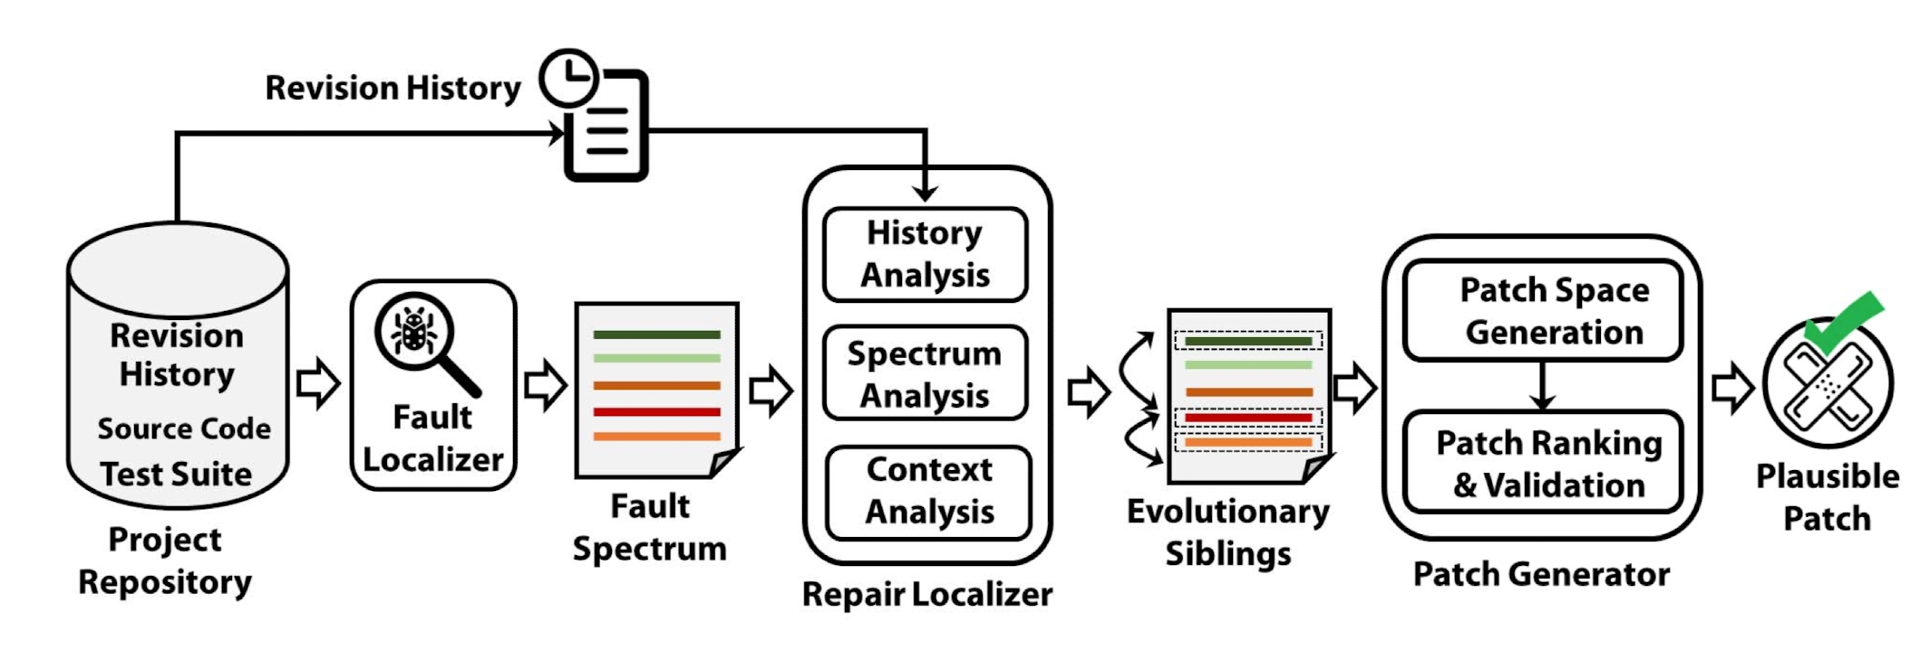
\includegraphics[width=\textwidth]{overview}
\caption{Overview of HERCULES.} \label{fig1}
\end{figure}

Previous techniques like ACS and SimFix can do simple multi-hunk repair. However, these tools simply continuously repair bugs independently one by one, since bugs are revealed by individual test cases separately. In this scenario, the search space of repair locations is going to grow exponentially, though it is viable for the simplest cases \cite{0_ref_proc1}.

By comparison, the HERCULES approach utilizes the relationship between siblings to effectively maintain the search space identical to that of a single-hunk repair. It uses reaching definition analysis, abstract syntax tree (AST) analysis and revision history to identify and revise evolutionary siblings \cite{0_ref_proc1}. Based on the results from the last step, HERCULES generates a multi-hunk or a single patch\cite{0_ref_proc1}. Following that, HERCULES employs ranking models to prioritize candidate patches and selects the top N for validation \cite{0_ref_proc1}. For each candidate patch, HERCULES initially executes failing tests; if they pass, regression tests are then conducted. If both sets of tests pass, HERCULES identifies the patch as the final correct patch and concludes the process \cite{0_ref_proc1}.
Table~\ref{tab1} shows the statistics of correct and incorrect patches generated by different techniques.

\begin{table}
\centering
\caption{Numbers of Patch Generation by Various Techniques (Correct/incorrect)}\label{tab1}
\begin{tabular}{l l l l l l l}
\hline
{\bfseries Subject} &  {\bfseries Math} & {\bfseries Lang} & {\bfseries Time} & {\bfseries Chart} & {\bfseries Closure} & {\bfseries Total}\\
\hline
HERCULES &  21/7 & 10/3 & 3/2 & 6/3 & 6/2 & \colorbox{lightgray} {\bfseries46/17}\\
SimFix &  14/12 & 9/4 & 1/0 & 4/4 & 6/2 & 34/22\\
CapGen &  13/- & 5/- & 0/- & 4/- & 0/- & 22/-\\
JAID &  1/- & 1/- & 0/- & 2/- & 5/- & 9/-\\
ELIXIR &  12/7 & 8/4 & 2/1 & 4/3 & 0/- & 26/15\\
ssFix &  10/16 & 5/7 & 0/4 & 3/4 & 2/9 & 20/40\\
ACS &  12/4 & 3/1 & 1/0 & 2/0 & 0/- & 18/5\\
% Title (centered) &  {\Large\bfseries Lecture Notes} & 14 point, bold\\
% 1st-level heading &  {\large\bfseries 1 Introduction} & 12 point, bold\\
% 2nd-level heading & {\bfseries 2.1 Printing Area} & 10 point, bold\\
% 3rd-level heading & {\bfseries Run-in Heading in Bold.} Text follows & 10 point, bold\\
% 4th-level heading & {\itshape Lowest Level Heading.} Text follows & 10 point, italic\\
\hline
\end{tabular}
\end{table}

\section{Future Suggestions}
Undeniably, expanding the validation of automatic program repair to encompass a broader range of subjects is crucial for future research. While the current focus on subjects like Math, Lang, Chart, Time, and Closure is necessary, it's evident that this scope is far from enough. Including additional subjects in future validation efforts will provide a more thorough understanding of the effectiveness and generalizability of automatic program repair techniques. It is fine that research in a new field starts from a small step first as long as future ones can achieve more progress. 

The problem of accuracy of version history analysis is a real obstacle that related researchers need to overcome. It is unavoidable that the structure of a project repository changes over time because of refactoring or upgrades. We need to find out the patterns in structural changes of any repository so that old versions of code can be retrieved from history, which in return improves our similarity comparison.

Since HERCULES is functional and more powerful than any other existing technique so far. Researchers should apply it to program repair of other programming languages. Some popular languages such as C/C++, python, C\# and JavaScript should be included at least. The truth is a project may use more than one language in its code, which is a challenge for future experiments.

\section{Critical Review}

\subsection{Good}
They did well at convincing readers that it is time to achieve the goal of the practical deployment of automatic program repair techniques. A significant hurdle lies in the incapacity of current APR techniques to generate multi-hunk patches. Technically, they address this challenge by extending single-hunk repair methodologies to encompass a particular yet significant category of multi-hunk repair issues. They use evolutionary siblings to name such sets of similar repair locations.

Clear explanations of terminology and definitions are given before the main body of the paper, followed by a motivating example introducing their method of experiment. The concrete experimental configurations are also stated clearly.
They listed four research questions before experimenting. In the results section, these questions are answered one by one with clear logic and plentiful evidence.

\subsection{Not Good Enough}
\begin{enumerate}
\item HERCULES is capable of executing one specific type of multi-hunk repair, which is insufficient to establish HERCULES or multi-hunk repair as a significant breakthrough. However, it does enhance successful repairs by nearly 50\% compared to certain previous tools.\\
\item Version history analysis is crucial, yet it can be impeded by noise in the repository's revision history. Major structural alterations to the directory or package, or other systemic refactoring changes, may obscure the tracking process. To mitigate these issues, researchers often employ heuristics to minimize the negative impact of exceptions and manually inspect the history of bug samples to validate accuracy. However, the reliability of version history analysis in this scenario is not guaranteed.\\
\item The results lack evidence of generalizability. The evaluation was exclusively carried out on the Defects4J dataset, which comprises only five subject systems. Consequently, these systems may not adequately represent the diverse range of Java applications and their associated bugs. Their technique has only been applied to Java program repair. Whether it can be applied to other programs’ repair and whether it is still effective and efficient are to be checked.\\
\item Their present multi-hunk repair technique is integrated into a baseline repair tool. While effective, the outcomes could potentially be enhanced by leveraging a more advanced APR tool.
\end{enumerate}

\subsection{My Method}
If I were the leader of this research team, I would perform more experiments and make more comparisons with other tools or techniques before analysing the results and drawing conclusions.
Considering the limitations of the current research, I would suggest that the team should apply HERCULES to other programming languages and more subjects since a project can be build of many languages.\\
The team should also improve the accuracy of version history analysis and the generalizability of the technique.
To improve the reliability of version history analysis, focus on mitigating the impact of noise in the repository's revision history. Develop more robust heuristics to handle major structural alterations or systemic refactoring changes effectively. Consider incorporating automated techniques for noise reduction and validation to ensure the accuracy and reliability of the analysis results.
To strengthen the generalizability of the evaluation results, consider expanding the dataset beyond the Defects4J dataset. Include a more diverse range of subject systems representing various Java applications and their associated bugs. Additionally, explore the applicability of the technique to repair programs written in languages other than Java to assess its effectiveness and efficiency in different contexts.\\
We should make as many improvements as possible before publishing a paper.

% ---- Bibliography ----
%
% BibTeX users should specify bibliography style 'splncs04'.
% References will then be sorted and formatted in the correct style.
%
% \bibliographystyle{agsm}
\bibliographystyle{splncs04}
% \bibliography{mybibliography}
%
\newpage
\begin{thebibliography}{8}
\bibitem{0_ref_proc1}
Saha, S., Saha, R.K., Prasad, M.R.: Harnessing Evolution for Multi-Hunk Program Repair. In: 2019 IEEE/ACM 41st International Conference on Software Engineering (ICSE)
on Proceedings, pp. 13--24. IEEE, America (2019)

\bibitem{1_ref_proc2}
Gazzola, L., Mariani, L., Micucci, D.: Automatic software repair: A survey. In: 2018 IEEE/ACM 40th International Conference on Software Engineering (ICSE)
on Proceedings, pp. 1--1. ACM (2018)

\bibitem{2_ref_article1}
Monperrus, M.: Automatic Software Repair: A Bibliography. ACM Computing Surveys \textbf{51}(1), 1--24 (2018)

\bibitem{3_ref_article2}
Le Goues, C., Forrest, S., Weimer, W.: Current challenges in automatic software repair. Software quality journal \textbf{21}(3), 421--443 (2013)

\bibitem{4_ref_proc3}
Zhong, H., Su, Z.: An Empirical Study on Real Bug Fixes. In: The Institute of Electrical and Electronics Engineers, Inc. (IEEE) Conference Proceedings
on Proceedings, pp. 913. Piscataway (2015)

\bibitem{5_ref_proc4}
Mechtaev, S., Yi, J., Roychoudhury, A.: Angelix: Scalable Multiline Program Patch Synthesis via Symbolic Analysis. In: 2016 IEEE/ACM 38th International Conference on Software Engineering (ICSE)
on Proceedings, pp. 691--701. ACM (2016)

\bibitem{6_ref_proc5}
Just, R., Jalali, D., Ernst, M.D.: Defects4J: a database of existing faults to enable controlled testing studies for Java programs. In: 2014 International Symposium on Software Testing and Analysis, ISSTA 2014 - Proceedings
on Proceedings, pp. 437--440. ACM (2014)

\bibitem{7_ref_proc6}
Saha, R.K., Lyu, Y., Lam, W., Yoshida, H., Prasad, M.R.: Bugs.jar: A Large-Scale, Diverse Dataset of Real-World Java Bugs. In: 15th International Conference on Mining Software Repositories
on Proceedings, pp. 10--13. ACM (2018)

\bibitem{8_ref_article3}
Kim, M., Notkin, D.: Using a clone genealogy extractor for understanding and supporting evolution of code clones. ACM SIGSOFT Software Engineering Notes \textbf{30}(4), 2--5 (2005)

\bibitem{9_ref_proc7}
Roy, C.K., Cordy, J.R.: An Empirical Study of Function Clones in Open Source Software. In: 15th Working Conference on Reverse Engineering
on Proceedings, pp. 81--90. IEEE (2008)

\bibitem{10_ref_proc8}
Duala-Ekoko, E., Robillard, M.P.: Tracking code clones in evolving software. In: Software Engineering 2007. ICSE 2007. 29th International Conference
on Proceedings, pp. 158--167.  IEEE Computer Society (2007)

\bibitem{11_ref_proc9}
Juergens, E.,Deissenboeck, F.,Hummel, B., Wagner, S.: Do code clones matter?. In: 2009 IEEE 31st International Conference on Software Engineering
on Proceedings, pp. 485--495. IEEE Computer Society (2009)

\bibitem{12_ref_article4}
Kamiya, T., Kusumoto, S., Inoue, K.: CCFinder: a multilinguistic token-based code clone detection system for large scale source code. IEEE Transactions on Software Engineering \textbf{28}(7), 654--670 (2002)

\bibitem{13_ref_proc10}
Jiang, L., Misherghi, G., Su, Z., Glondu, S.: Deckard: Scalable and accurate tree-based detection of code clones. In: 29th international conference on Software Engineering
on Proceedings, pp. 96--105. IEEE Computer Society (2007)

\bibitem{14_ref_proc11}
Cordy, J.R., Roy, C.K.: The NiCad Clone Detector. In: 2011 IEEE 19th International Conference on Program Comprehension
on Proceedings, pp. 219--220. IEEE (2011)

\bibitem{15_ref_proc12}
Meng, N., Kim, M., McKinley, K.S.: Systematic editing: Generating program transformations from an example. In: 32nd ACM SIGPLAN Conference on programming language design and implementation
on Proceedings, pp. 329--342. ACM (2011)

\bibitem{16_ref_proc13}
Meng, N., Kim, M., McKinley, K.S.: LASE: locating and applying systematic edits by learning from examples. In: 35th International Conference on Software Engineering (ICSE)
on Proceedings, pp. 502--511. IEEE (2013)

\bibitem{17_ref_proc14}
Meng, N., Hua, L., Kim, M., McKinley, K.S.: Does automated refactoring obviate systematic editing?. In: 37th International Conference on Software Engineering
on Proceedings, pp. 392--402. IEEE (2015)

\bibitem{20_ref_proc15}
Islam, J.F., Mondal, M., Roy, C.K.: Bug replication in code clones: An empirical study. In: Software Analysis Evolution and Reengineering (SANER) 2016 IEEE 23rd International Conference
on Proceedings, pp. 68--78. Piscataway (2016)

\bibitem{24_ref_proc16}
Tan, S.H., Yoshida, H., Prasad, M.R., Roychoudhury, A.: Anti-patterns in search-based program repair. In: 2016 24th ACM SIGSOFT International Symposium on Foundations of Software Engineering
on Proceedings, pp. 727--738. ACM (2016)

\bibitem{27_ref_proc17}
Jiang, J., Xiong, Y., Zhang, H., Gao, Q., Chen, X.: Shaping program repair space with existing patches and similar code. In: 27th ACM SIGSOFT International Symposium on Software Testing and Analysis
on Proceedings, pp. 298--309. (2018)

\bibitem{28_ref_proc18}
Le Goues, C., Dewey-Vogt, M., Forrest, S., Weimer, W.: A systematic study of automated program repair: Fixing 55 out of 105 bugs for \$8 each. In: 34th International Conference on Software Engineering
on Proceedings, pp. 3--13. IEEE (2012)

\bibitem{29_ref_proc19}
Xiong, Y., Wang, J., Yan, R., Zhang, J., Han, S., Huang, G., Zhang, L.: Precise Condition Synthesis for Program Repair. In: 39th International Conference on Software Engineering (ICSE)
on Proceedings, pp. 416--426. IEEE (2017)

\bibitem{30_ref_proc20}
Xin, Q., Resis, S.P.: Leveraging syntax-related code for automated program repair. In: 32nd IEEE/ACM International Conference on Automated Software Engineering
on Proceedings, pp. 660--670. Piscataway (2017)

% %%%%%%%%%%%%%%%%%%%%%%%%%%%%%%%%%%%%%%%%%%%%%%%%%%%%%%%%%%%%%%%%%%%%%%%%%%%%%
% \bibitem{ref_article}
% Author, F.: Article title. Journal \textbf{2}(5), 99--110 (2016)

% \bibitem{ref_lncs1}
% Author, F., Author, S.: Title of a proceedings paper. In: Editor,
% F., Editor, S. (eds.) CONFERENCE 2016, LNCS, vol. 9999, pp. 1--13.
% Springer, Heidelberg (2016). \doi{10.10007/1234567890}

% \bibitem{ref_book1}
% Author, F., Author, S., Author, T.: Book title. 2nd edn. Publisher,
% Location (1999)

% \bibitem{ref_proc}
% Author, A.-B.: Contribution title. In: 9th International Proceedings
% on Proceedings, pp. 1--2. Publisher, Location (2010)

% \bibitem{ref_url1}
% LNCS Homepage, \url{http://www.springer.com/lncs}, last accessed 2023/10/25
\end{thebibliography}
\end{document}
